%!TEX root = ../dokumentation.tex

\chapter{package.json}
\label{ch:package.json}
Die package.json Datei beinhaltet die grundlegenden Informationen zur Anwendung. Dazu gehören allgemeine Informationen, eigene Skripte und die Abhängigkeiten der Anwendung von anderen Frameworks und Softwarepaketen

\begin{wrapfigure}{r}{0\textwidth}
\centering
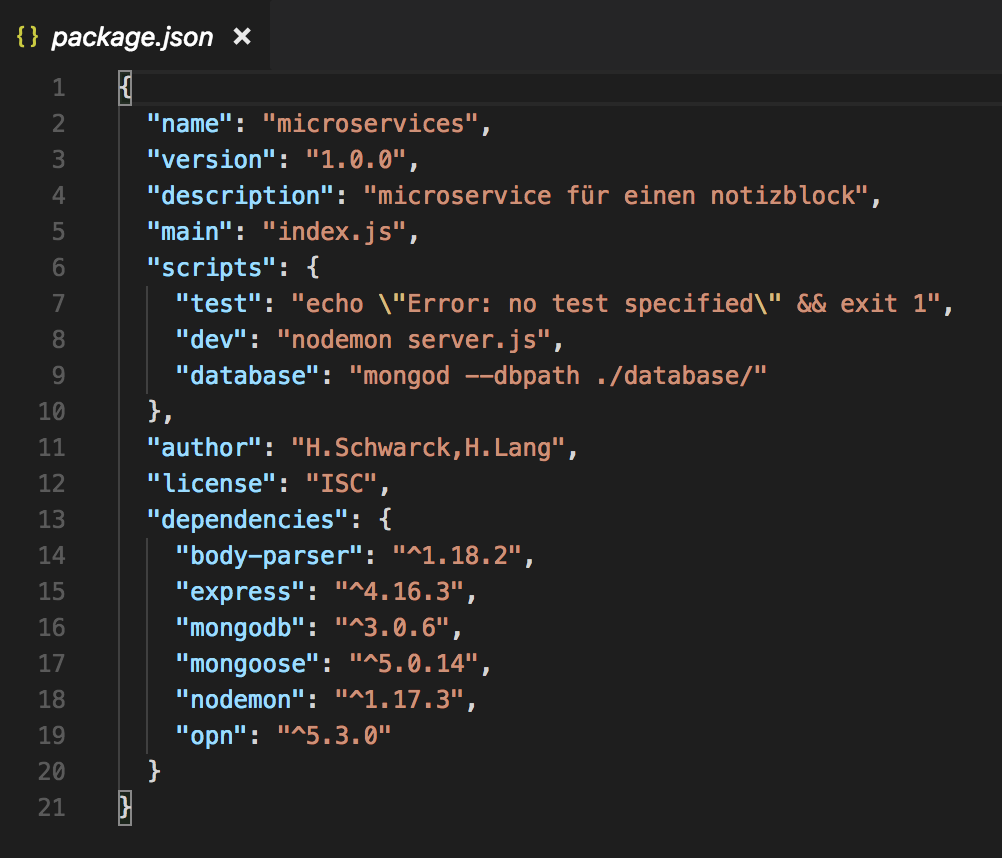
\includegraphics[height=.5\textwidth]{Packagejson.png}
\vspace{4pt}
\caption{Dependencies der package.json}
\label{fig:Dependencies der package.json}
\end{wrapfigure}

Wie in der Abbildung zu sehen beginnt die Datei mit den allgemeinen Informationen über die Anwendung. Dazu gehören der Name der Anwendung, die Version, eine kurze Beschreibung, der Einstiegspunkt der Anwendung, selbstdefinierte Skripte zur Ausführung, die Namen der Entwickler und die Lizenz.

Danach werden die Dependencies, also die Abhängigkeiten, aufgelistet. Diese beschreiben die verwendeten Frameworks auf die die Anwendung zurückgreift.

Durch den \glqq NodePackageManager\grqq{} können diese Abhängigkeiten aufgelöst und in das System importiert werden. Dies geschieht durch den Befehl npm install der auch in der Dockerfile zu finden ist.